% Options for packages loaded elsewhere
% Options for packages loaded elsewhere
\PassOptionsToPackage{unicode}{hyperref}
\PassOptionsToPackage{hyphens}{url}
\PassOptionsToPackage{dvipsnames,svgnames,x11names}{xcolor}
%
\documentclass[
  letterpaper,
  DIV=11,
  numbers=noendperiod]{scrartcl}
\usepackage{xcolor}
\usepackage{amsmath,amssymb}
\setcounter{secnumdepth}{-\maxdimen} % remove section numbering
\usepackage{iftex}
\ifPDFTeX
  \usepackage[T1]{fontenc}
  \usepackage[utf8]{inputenc}
  \usepackage{textcomp} % provide euro and other symbols
\else % if luatex or xetex
  \usepackage{unicode-math} % this also loads fontspec
  \defaultfontfeatures{Scale=MatchLowercase}
  \defaultfontfeatures[\rmfamily]{Ligatures=TeX,Scale=1}
\fi
\usepackage{lmodern}
\ifPDFTeX\else
  % xetex/luatex font selection
\fi
% Use upquote if available, for straight quotes in verbatim environments
\IfFileExists{upquote.sty}{\usepackage{upquote}}{}
\IfFileExists{microtype.sty}{% use microtype if available
  \usepackage[]{microtype}
  \UseMicrotypeSet[protrusion]{basicmath} % disable protrusion for tt fonts
}{}
\makeatletter
\@ifundefined{KOMAClassName}{% if non-KOMA class
  \IfFileExists{parskip.sty}{%
    \usepackage{parskip}
  }{% else
    \setlength{\parindent}{0pt}
    \setlength{\parskip}{6pt plus 2pt minus 1pt}}
}{% if KOMA class
  \KOMAoptions{parskip=half}}
\makeatother
% Make \paragraph and \subparagraph free-standing
\makeatletter
\ifx\paragraph\undefined\else
  \let\oldparagraph\paragraph
  \renewcommand{\paragraph}{
    \@ifstar
      \xxxParagraphStar
      \xxxParagraphNoStar
  }
  \newcommand{\xxxParagraphStar}[1]{\oldparagraph*{#1}\mbox{}}
  \newcommand{\xxxParagraphNoStar}[1]{\oldparagraph{#1}\mbox{}}
\fi
\ifx\subparagraph\undefined\else
  \let\oldsubparagraph\subparagraph
  \renewcommand{\subparagraph}{
    \@ifstar
      \xxxSubParagraphStar
      \xxxSubParagraphNoStar
  }
  \newcommand{\xxxSubParagraphStar}[1]{\oldsubparagraph*{#1}\mbox{}}
  \newcommand{\xxxSubParagraphNoStar}[1]{\oldsubparagraph{#1}\mbox{}}
\fi
\makeatother

\usepackage{color}
\usepackage{fancyvrb}
\newcommand{\VerbBar}{|}
\newcommand{\VERB}{\Verb[commandchars=\\\{\}]}
\DefineVerbatimEnvironment{Highlighting}{Verbatim}{commandchars=\\\{\}}
% Add ',fontsize=\small' for more characters per line
\usepackage{framed}
\definecolor{shadecolor}{RGB}{241,243,245}
\newenvironment{Shaded}{\begin{snugshade}}{\end{snugshade}}
\newcommand{\AlertTok}[1]{\textcolor[rgb]{0.68,0.00,0.00}{#1}}
\newcommand{\AnnotationTok}[1]{\textcolor[rgb]{0.37,0.37,0.37}{#1}}
\newcommand{\AttributeTok}[1]{\textcolor[rgb]{0.40,0.45,0.13}{#1}}
\newcommand{\BaseNTok}[1]{\textcolor[rgb]{0.68,0.00,0.00}{#1}}
\newcommand{\BuiltInTok}[1]{\textcolor[rgb]{0.00,0.23,0.31}{#1}}
\newcommand{\CharTok}[1]{\textcolor[rgb]{0.13,0.47,0.30}{#1}}
\newcommand{\CommentTok}[1]{\textcolor[rgb]{0.37,0.37,0.37}{#1}}
\newcommand{\CommentVarTok}[1]{\textcolor[rgb]{0.37,0.37,0.37}{\textit{#1}}}
\newcommand{\ConstantTok}[1]{\textcolor[rgb]{0.56,0.35,0.01}{#1}}
\newcommand{\ControlFlowTok}[1]{\textcolor[rgb]{0.00,0.23,0.31}{\textbf{#1}}}
\newcommand{\DataTypeTok}[1]{\textcolor[rgb]{0.68,0.00,0.00}{#1}}
\newcommand{\DecValTok}[1]{\textcolor[rgb]{0.68,0.00,0.00}{#1}}
\newcommand{\DocumentationTok}[1]{\textcolor[rgb]{0.37,0.37,0.37}{\textit{#1}}}
\newcommand{\ErrorTok}[1]{\textcolor[rgb]{0.68,0.00,0.00}{#1}}
\newcommand{\ExtensionTok}[1]{\textcolor[rgb]{0.00,0.23,0.31}{#1}}
\newcommand{\FloatTok}[1]{\textcolor[rgb]{0.68,0.00,0.00}{#1}}
\newcommand{\FunctionTok}[1]{\textcolor[rgb]{0.28,0.35,0.67}{#1}}
\newcommand{\ImportTok}[1]{\textcolor[rgb]{0.00,0.46,0.62}{#1}}
\newcommand{\InformationTok}[1]{\textcolor[rgb]{0.37,0.37,0.37}{#1}}
\newcommand{\KeywordTok}[1]{\textcolor[rgb]{0.00,0.23,0.31}{\textbf{#1}}}
\newcommand{\NormalTok}[1]{\textcolor[rgb]{0.00,0.23,0.31}{#1}}
\newcommand{\OperatorTok}[1]{\textcolor[rgb]{0.37,0.37,0.37}{#1}}
\newcommand{\OtherTok}[1]{\textcolor[rgb]{0.00,0.23,0.31}{#1}}
\newcommand{\PreprocessorTok}[1]{\textcolor[rgb]{0.68,0.00,0.00}{#1}}
\newcommand{\RegionMarkerTok}[1]{\textcolor[rgb]{0.00,0.23,0.31}{#1}}
\newcommand{\SpecialCharTok}[1]{\textcolor[rgb]{0.37,0.37,0.37}{#1}}
\newcommand{\SpecialStringTok}[1]{\textcolor[rgb]{0.13,0.47,0.30}{#1}}
\newcommand{\StringTok}[1]{\textcolor[rgb]{0.13,0.47,0.30}{#1}}
\newcommand{\VariableTok}[1]{\textcolor[rgb]{0.07,0.07,0.07}{#1}}
\newcommand{\VerbatimStringTok}[1]{\textcolor[rgb]{0.13,0.47,0.30}{#1}}
\newcommand{\WarningTok}[1]{\textcolor[rgb]{0.37,0.37,0.37}{\textit{#1}}}

\usepackage{longtable,booktabs,array}
\newcounter{none} % for unnumbered tables
\usepackage{calc} % for calculating minipage widths
% Correct order of tables after \paragraph or \subparagraph
\usepackage{etoolbox}
\makeatletter
\patchcmd\longtable{\par}{\if@noskipsec\mbox{}\fi\par}{}{}
\makeatother
% Allow footnotes in longtable head/foot
\IfFileExists{footnotehyper.sty}{\usepackage{footnotehyper}}{\usepackage{footnote}}
\makesavenoteenv{longtable}
\usepackage{graphicx}
\makeatletter
\newsavebox\pandoc@box
\newcommand*\pandocbounded[1]{% scales image to fit in text height/width
  \sbox\pandoc@box{#1}%
  \Gscale@div\@tempa{\textheight}{\dimexpr\ht\pandoc@box+\dp\pandoc@box\relax}%
  \Gscale@div\@tempb{\linewidth}{\wd\pandoc@box}%
  \ifdim\@tempb\p@<\@tempa\p@\let\@tempa\@tempb\fi% select the smaller of both
  \ifdim\@tempa\p@<\p@\scalebox{\@tempa}{\usebox\pandoc@box}%
  \else\usebox{\pandoc@box}%
  \fi%
}
% Set default figure placement to htbp
\def\fps@figure{htbp}
\makeatother





\setlength{\emergencystretch}{3em} % prevent overfull lines

\providecommand{\tightlist}{%
  \setlength{\itemsep}{0pt}\setlength{\parskip}{0pt}}



 


\KOMAoption{captions}{tableheading}
\makeatletter
\@ifpackageloaded{caption}{}{\usepackage{caption}}
\AtBeginDocument{%
\ifdefined\contentsname
  \renewcommand*\contentsname{Table of contents}
\else
  \newcommand\contentsname{Table of contents}
\fi
\ifdefined\listfigurename
  \renewcommand*\listfigurename{List of Figures}
\else
  \newcommand\listfigurename{List of Figures}
\fi
\ifdefined\listtablename
  \renewcommand*\listtablename{List of Tables}
\else
  \newcommand\listtablename{List of Tables}
\fi
\ifdefined\figurename
  \renewcommand*\figurename{Figure}
\else
  \newcommand\figurename{Figure}
\fi
\ifdefined\tablename
  \renewcommand*\tablename{Table}
\else
  \newcommand\tablename{Table}
\fi
}
\@ifpackageloaded{float}{}{\usepackage{float}}
\floatstyle{ruled}
\@ifundefined{c@chapter}{\newfloat{codelisting}{h}{lop}}{\newfloat{codelisting}{h}{lop}[chapter]}
\floatname{codelisting}{Listing}
\newcommand*\listoflistings{\listof{codelisting}{List of Listings}}
\makeatother
\makeatletter
\makeatother
\makeatletter
\@ifpackageloaded{caption}{}{\usepackage{caption}}
\@ifpackageloaded{subcaption}{}{\usepackage{subcaption}}
\makeatother
\usepackage{bookmark}
\IfFileExists{xurl.sty}{\usepackage{xurl}}{} % add URL line breaks if available
\urlstyle{same}
\hypersetup{
  pdftitle={Assignment ØKA201 Data Analysis},
  pdfauthor={Arvid Thapa Strand},
  colorlinks=true,
  linkcolor={blue},
  filecolor={Maroon},
  citecolor={Blue},
  urlcolor={Blue},
  pdfcreator={LaTeX via pandoc}}


\title{Assignment ØKA201 Data Analysis}
\author{Arvid Thapa Strand}
\date{2026-05-01}
\begin{document}
\maketitle

\renewcommand*\contentsname{Table of contents}
{
\setcounter{tocdepth}{3}
\tableofcontents
}
\listoffigures
\listoftables

\section{Abstract}\label{abstract}

This paper investigates how reading and writing performance are
associated with mathematics achievement among students. Using regression
analysis in R, several econometric models are estimated and compared,
including simple regression, multiple regression, dummy variable
analysis, and non-linear specifications. The findings suggest that
reading and writing scores are positively related to mathematics
performance.

\textbf{Keywords:} regression analysis, R programming, student
performance, mathematics, Quarto

\section{Introduction}\label{introduction}

The purpose of this paper is to analyze factors affecting student
performance using regression analysis in R. The analysis focuses on the
relationship between reading, writing, and mathematics scores using the
Students Performance dataset from Kaggle.

The paper builds upon the previous Gretl assignment and replicates the
econometric analysis in R. According to (\textbf{wickham2017r?}), R
provides flexible tools for statistical computing, data wrangling, and
visualization which are useful for empirical economic analysis.

\section{1. Research Question}\label{research-question}

The research question is:

\emph{How are reading and writing scores associated with mathematics
performance among students?}

\section{2. Data Set}\label{data-set}

The dataset used in this analysis is the Students Performance dataset
from Kaggle. The dataset contains information about gender, parental
education, lunch type, test preparation course, and student exam scores
in mathematics, reading, and writing.

\section{3. Data Description and
Summary}\label{data-description-and-summary}

\begin{verbatim}
  gender race.ethnicity parental.level.of.education        lunch
1 female        group B           bachelor's degree     standard
2 female        group C                some college     standard
3 female        group B             master's degree     standard
4   male        group A          associate's degree free/reduced
5   male        group C                some college     standard
6 female        group B          associate's degree     standard
  test.preparation.course math.score reading.score writing.score
1                    none         72            72            74
2               completed         69            90            88
3                    none         90            95            93
4                    none         47            57            44
5                    none         76            78            75
6                    none         71            83            78
\end{verbatim}

\begin{verbatim}
    gender          race.ethnicity     parental.level.of.education
 Length:1000        Length:1000        Length:1000                
 Class :character   Class :character   Class :character           
 Mode  :character   Mode  :character   Mode  :character           
                                                                  
                                                                  
                                                                  
    lunch           test.preparation.course   math.score     reading.score   
 Length:1000        Length:1000             Min.   :  0.00   Min.   : 17.00  
 Class :character   Class :character        1st Qu.: 57.00   1st Qu.: 59.00  
 Mode  :character   Mode  :character        Median : 66.00   Median : 70.00  
                                            Mean   : 66.09   Mean   : 69.17  
                                            3rd Qu.: 77.00   3rd Qu.: 79.00  
                                            Max.   :100.00   Max.   :100.00  
 writing.score   
 Min.   : 10.00  
 1st Qu.: 57.75  
 Median : 69.00  
 Mean   : 68.05  
 3rd Qu.: 79.00  
 Max.   :100.00  
\end{verbatim}

The dataset contains 1000 observations of student performance. The
average mathematics score is approximately 66, while the average reading
score is approximately 69.

\section{4. Scatterplot Analysis}\label{scatterplot-analysis}

\begin{figure}

\centering{

\pandocbounded{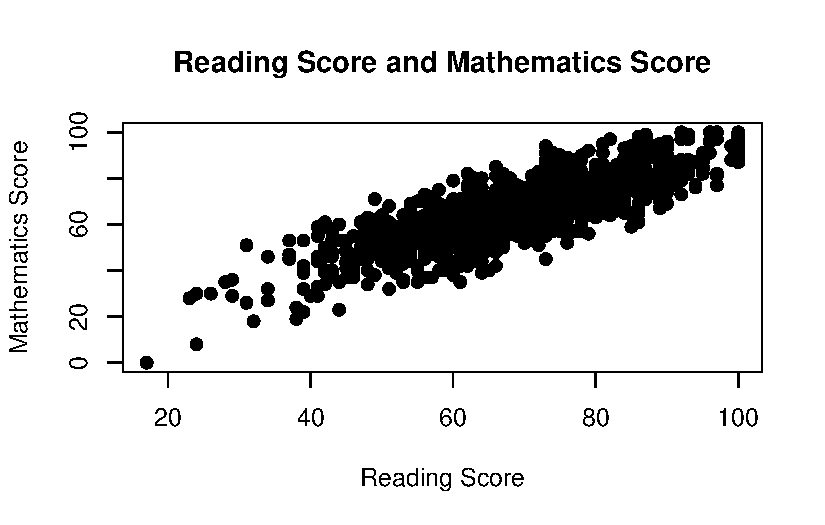
\includegraphics[keepaspectratio]{assignment_r_files/figure-pdf/fig-scatter-1.pdf}}

}

\caption{\label{fig-scatter}Scatterplot of reading and mathematics
scores}

\end{figure}%

The scatterplot suggests a positive relationship between reading scores
and mathematics scores.

\section{5. Simple Regression Model}\label{simple-regression-model}

\begin{verbatim}

Call:
lm(formula = math.score ~ reading.score, data = data)

Residuals:
     Min       1Q   Median       3Q      Max 
-24.3419  -6.3419  -0.0221   6.2713  24.6581 

Coefficients:
              Estimate Std. Error t value Pr(>|t|)    
(Intercept)    7.35759    1.33818   5.498 4.87e-08 ***
reading.score  0.84910    0.01893  44.855  < 2e-16 ***
---
Signif. codes:  0 '***' 0.001 '**' 0.01 '*' 0.05 '.' 0.1 ' ' 1

Residual standard error: 8.736 on 998 degrees of freedom
Multiple R-squared:  0.6684,    Adjusted R-squared:  0.6681 
F-statistic:  2012 on 1 and 998 DF,  p-value: < 2.2e-16
\end{verbatim}

The estimated coefficient for reading score is positive and
statistically significant at the 5 percent significance level. This
indicates that higher reading performance is associated with higher
mathematics scores.

\section{6. Multiple Regression Model}\label{multiple-regression-model}

\begin{verbatim}

Call:
lm(formula = math.score ~ reading.score + writing.score, data = data)

Residuals:
     Min       1Q   Median       3Q      Max 
-23.8779  -6.1750   0.2693   6.0184  24.8727 

Coefficients:
              Estimate Std. Error t value Pr(>|t|)    
(Intercept)    7.52409    1.32823   5.665 1.93e-08 ***
reading.score  0.60129    0.06304   9.538  < 2e-16 ***
writing.score  0.24942    0.06057   4.118 4.14e-05 ***
---
Signif. codes:  0 '***' 0.001 '**' 0.01 '*' 0.05 '.' 0.1 ' ' 1

Residual standard error: 8.667 on 997 degrees of freedom
Multiple R-squared:  0.674, Adjusted R-squared:  0.6733 
F-statistic:  1031 on 2 and 997 DF,  p-value: < 2.2e-16
\end{verbatim}

The multiple regression model includes both reading and writing scores
as explanatory variables. Both variables contribute positively to
mathematics performance.

\section{7. Dummy Variable Analysis}\label{dummy-variable-analysis}

\begin{verbatim}

Call:
lm(formula = math.score ~ reading.score + female, data = data)

Residuals:
     Min       1Q   Median       3Q      Max 
-22.7447  -4.3918  -0.0747   4.1590  18.1338 

Coefficients:
              Estimate Std. Error t value Pr(>|t|)    
(Intercept)     6.6384     1.0078   6.587 7.26e-11 ***
reading.score   0.9483     0.0147  64.523  < 2e-16 ***
female        -11.8614     0.4292 -27.634  < 2e-16 ***
---
Signif. codes:  0 '***' 0.001 '**' 0.01 '*' 0.05 '.' 0.1 ' ' 1

Residual standard error: 6.577 on 997 degrees of freedom
Multiple R-squared:  0.8122,    Adjusted R-squared:  0.8119 
F-statistic:  2157 on 2 and 997 DF,  p-value: < 2.2e-16
\end{verbatim}

The dummy variable captures differences between male and female
students. The coefficient for the female variable is statistically
significant, indicating systematic differences between groups.

\section{8. Non-linear Effects}\label{non-linear-effects}

\begin{verbatim}

Call:
lm(formula = math.score ~ reading.score + I(reading.score^2), 
    data = data)

Residuals:
     Min       1Q   Median       3Q      Max 
-24.4463  -6.3301   0.0727   6.2636  24.5537 

Coefficients:
                     Estimate Std. Error t value Pr(>|t|)    
(Intercept)         4.9091162  4.3148582   1.138    0.256    
reading.score       0.9255394  0.1294523   7.150 1.68e-12 ***
I(reading.score^2) -0.0005681  0.0009517  -0.597    0.551    
---
Signif. codes:  0 '***' 0.001 '**' 0.01 '*' 0.05 '.' 0.1 ' ' 1

Residual standard error: 8.738 on 997 degrees of freedom
Multiple R-squared:  0.6686,    Adjusted R-squared:  0.6679 
F-statistic:  1006 on 2 and 997 DF,  p-value: < 2.2e-16
\end{verbatim}

The non-linear model includes a quadratic term for reading score. The
quadratic term is not strongly significant, suggesting that the
relationship is approximately linear.

\section{9. Model Comparison}\label{model-comparison}

{

\begin{longtable}[]{@{}lr@{}}

\caption{\label{tbl-models}Model comparison: R-squared values}

\tabularnewline

\toprule\noalign{}
Model & R\_squared \\
\midrule\noalign{}
\endhead
\bottomrule\noalign{}
\endlastfoot
Simple Regression & 0.6684 \\
Multiple Regression & 0.6740 \\
Dummy Variable & 0.8122 \\
Non-linear & 0.6686 \\

\end{longtable}

}

The multiple regression model provides the best balance of explanatory
power and theoretical relevance.

\section{Conclusion}\label{conclusion}

The analysis indicates a positive relationship between reading
performance and mathematics performance. Reading and writing skills are
important predictors of student outcomes in mathematics. The multiple
regression model provided the most useful explanation of student
mathematics performance in this dataset.

\section{Word Count}\label{word-count}

\begin{Shaded}
\begin{Highlighting}[]
\NormalTok{word\_count }\OtherTok{\textless{}{-}} \ControlFlowTok{function}\NormalTok{(file) \{}
\NormalTok{  text }\OtherTok{\textless{}{-}} \FunctionTok{readLines}\NormalTok{(file)}
\NormalTok{  text }\OtherTok{\textless{}{-}} \FunctionTok{paste}\NormalTok{(text, }\AttributeTok{collapse =} \StringTok{" "}\NormalTok{)}
\NormalTok{  words }\OtherTok{\textless{}{-}} \FunctionTok{strsplit}\NormalTok{(text, }\StringTok{"}\SpecialCharTok{\textbackslash{}\textbackslash{}}\StringTok{s+"}\NormalTok{)[[}\DecValTok{1}\NormalTok{]]}
  \FunctionTok{length}\NormalTok{(words)}
\NormalTok{\}}
\FunctionTok{word\_count}\NormalTok{(}\StringTok{"assignment\_r.qmd"}\NormalTok{)}
\end{Highlighting}
\end{Shaded}

\begin{verbatim}
[1] 721
\end{verbatim}

\section{References}\label{references}

\protect\phantomsection\label{refs}

\section{Appendix: estm.R}\label{appendix-estm.r}

\begin{Shaded}
\begin{Highlighting}[]
\FunctionTok{library}\NormalTok{(tidyverse)}

\NormalTok{data }\OtherTok{\textless{}{-}} \FunctionTok{read.csv}\NormalTok{(}\StringTok{"data/student\_performance.csv"}\NormalTok{)}

\NormalTok{model1 }\OtherTok{\textless{}{-}} \FunctionTok{lm}\NormalTok{(math.score }\SpecialCharTok{\textasciitilde{}}\NormalTok{ reading.score, }\AttributeTok{data=}\NormalTok{data)}
\FunctionTok{summary}\NormalTok{(model1)}

\NormalTok{model2 }\OtherTok{\textless{}{-}} \FunctionTok{lm}\NormalTok{(math.score }\SpecialCharTok{\textasciitilde{}}\NormalTok{ reading.score }\SpecialCharTok{+}\NormalTok{ writing.score, }\AttributeTok{data=}\NormalTok{data)}
\FunctionTok{summary}\NormalTok{(model2)}

\NormalTok{data}\SpecialCharTok{$}\NormalTok{female }\OtherTok{\textless{}{-}} \FunctionTok{ifelse}\NormalTok{(data}\SpecialCharTok{$}\NormalTok{gender }\SpecialCharTok{==} \StringTok{"female"}\NormalTok{, }\DecValTok{1}\NormalTok{, }\DecValTok{0}\NormalTok{)}

\NormalTok{model3 }\OtherTok{\textless{}{-}} \FunctionTok{lm}\NormalTok{(math.score }\SpecialCharTok{\textasciitilde{}}\NormalTok{ reading.score }\SpecialCharTok{+}\NormalTok{ female, }\AttributeTok{data=}\NormalTok{data)}
\FunctionTok{summary}\NormalTok{(model3)}

\NormalTok{model4 }\OtherTok{\textless{}{-}} \FunctionTok{lm}\NormalTok{(math.score }\SpecialCharTok{\textasciitilde{}}\NormalTok{ reading.score }\SpecialCharTok{+} \FunctionTok{I}\NormalTok{(reading.score}\SpecialCharTok{\^{}}\DecValTok{2}\NormalTok{), }\AttributeTok{data=}\NormalTok{data)}
\FunctionTok{summary}\NormalTok{(model4)}
\end{Highlighting}
\end{Shaded}





\end{document}
